\documentclass[a4paper]{article}

%% Language and font encodings
\usepackage[english]{babel}
\usepackage[utf8x]{inputenc}
\usepackage[T1]{fontenc}

%% Sets page size and margins
\usepackage[a4paper,top=3cm,bottom=2cm,left=3cm,right=3cm,marginparwidth=1.75cm]{geometry}

%% Useful packages
\usepackage{amsmath}
\usepackage{graphicx}
\usepackage[colorinlistoftodos]{todonotes}
\usepackage[colorlinks=true, allcolors=blue]{hyperref}
\usepackage{listings}
\usepackage{minted}
\usepackage{tikz-qtree}

%% Title
\title{Traversal of Binary Trees}
\author{Khalid Hourani}

\begin{document}
There are four ways to traverse a binary tree. They are


\section{Pre-order Traversal}
To traverse a binary tree with a Pre-Order Traversal, begin at the root of the tree:
\begin{enumerate}
	\item If the current node has no children, stop.
    \item If the node has children:
    \begin{itemize}\item visit the \textbf{left  child} of the node. Repeat the algorithm on this subtree.
    				\item visit the \textbf{right child} of the node. Repeat this algorithm on this subtree.
	\end{itemize}
\end{enumerate}
\section{Post-order Traversal}
\section{In-order Traversal}
\section{Euler Tour Traversal}

\center
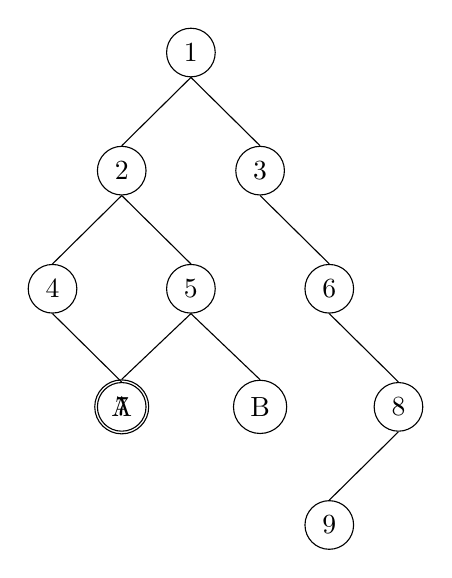
\begin{tikzpicture}[sibling distance=5em, every node/.style = {shape=circle, draw, align=center}]
\node {1}
	child { node {2}
    	child { node {4}
        	child[missing] { node {} }
        	child { node {7} }
        }
        child { node {5}
        child { node {A}}
        child { node {B}}
        }
    }
    child { node {3}
    	child[missing] { node {} }
        child { node {6}
        	child[missing] { node {} }
            child { node {8}
            child { node {9} }
            child[missing] { node {} }}
            }
    };
\end{tikzpicture}
\end{document}
